% -*- coding: utf-8 -*-
\documentclass[10pt,serif,t]{beamer}
\usepackage{times}
\usepackage[T1]{fontenc}
\usepackage{fancybox}
\usepackage{amsthm}
\usepackage{amsmath}
\usepackage{amsfonts}
\usepackage{graphicx}
\usepackage{subfigure}
\usepackage[adobefonts]{ctex} 

\uselanguage{TraditionalChinese}
\languagepath{TraditionalChinese}
\setbeamertemplate{caption}[numbered]

\usetheme{Madrid}

\newcommand*{\ket}[1]{\left\vert{#1}\right\rangle}
\newcommand{\cell}[3]{\parbox[c][#2][c]{#1}{\makebox[#1]{#3}}} 

\title{\heiti{}測試beamer文檔類的繁體中文翻譯}
\author{\songti{}胡海星}
\institute{\kaishu{}計算機科學與技術系\\
           南京大學}
\date{\today}

\begin{document}
%%%%%%%%%%%%%%%%%%%%%%%%%%%%%%%%%%%%%%%%%%%%%%%%%%%%%%%%%%%%%%%%%%%%%%%%%%%%%%%

\begin{frame}
    \titlepage
\end{frame}

\begin{frame}
  \frametitle{目錄}
  \tableofcontents
\end{frame}

\section{第一節}

\subsection{第一小節}

\begin{frame}
  \frametitle{測試定理環境}
  \begin{theorem}
    測試測試測試測試測試測試測試測試測試測試測試測試測試測試測試測試,
    測試測試測試測試測試測試測試測試測試測試。測試測試測試測試測試測試,
    測試測試測試測試測試測試測試測試。
  \end{theorem}
  \begin{proof}
    證明證明證明證明證明證明證明,證明證明證明證明證明證明證明。證明證明證明證明,
    證明證明證明證明證明證明證明。
  \end{proof}
\end{frame}

\subsection{第二小節}

\begin{frame}
  \frametitle{測試引理環境}
  \begin{lemma}
    測試測試測試測試測試測試測試測試測試測試測試測試測試測試測試測試,
    測試測試測試測試測試測試測試測試測試測試。測試測試測試測試測試測試,
    測試測試測試測試測試測試測試測試。
  \end{lemma}
  \begin{proof}
    證明證明證明證明證明證明證明,證明證明證明證明證明證明證明。證明證明證明證明,
    證明證明證明證明證明證明證明。
  \end{proof}
\end{frame}

\section{第二節}

\subsection{第一小節}

\begin{frame}
  \frametitle{測試例子環境}
  \begin{example}
    測試測試測試測試測試測試測試測試測試測試測試測試測試測試測試測試,
    測試測試測試測試測試測試測試測試測試測試。測試測試測試測試測試測試,
    測試測試測試測試測試測試測試測試。
  \end{example}
\end{frame}

\subsection{第二小節}

\begin{frame}
  \frametitle{測試推論環境}
  \begin{corollary}
    測試測試測試測試測試測試測試測試測試測試測試測試測試測試測試測試,
    測試測試測試測試測試測試測試測試測試測試。測試測試測試測試測試測試,
    測試測試測試測試測試測試測試測試。
  \end{corollary}
\end{frame}

\section{第三節}

\subsection{第一小節}

\begin{frame}
  \frametitle{測試定義環境}
  \begin{definition}
    測試測試測試測試測試測試測試測試測試測試測試測試測試測試測試測試,
    測試測試測試測試測試測試測試測試測試測試。測試測試測試測試測試測試,
    測試測試測試測試測試測試測試測試。
  \end{definition}
\end{frame}

\subsection{第二小節}

\begin{frame}
  \frametitle{測試事實環境}
  \begin{fact}
    測試測試測試測試測試測試測試測試測試測試測試測試測試測試測試測試,
    測試測試測試測試測試測試測試測試測試測試。測試測試測試測試測試測試,
    測試測試測試測試測試測試測試測試。
  \end{fact}
\end{frame}

\begin{frame}
  \frametitle{測試定義環境}
  \begin{definition}
    測試測試測試測試測試測試測試測試測試測試測試測試測試測試測試測試,
    測試測試測試測試測試測試測試測試測試測試。測試測試測試測試測試測試,
    測試測試測試測試測試測試測試測試。
  \end{definition}
\end{frame}

\begin{frame}
  \frametitle{測試插圖}  
  \begin{figure}
    \centering
    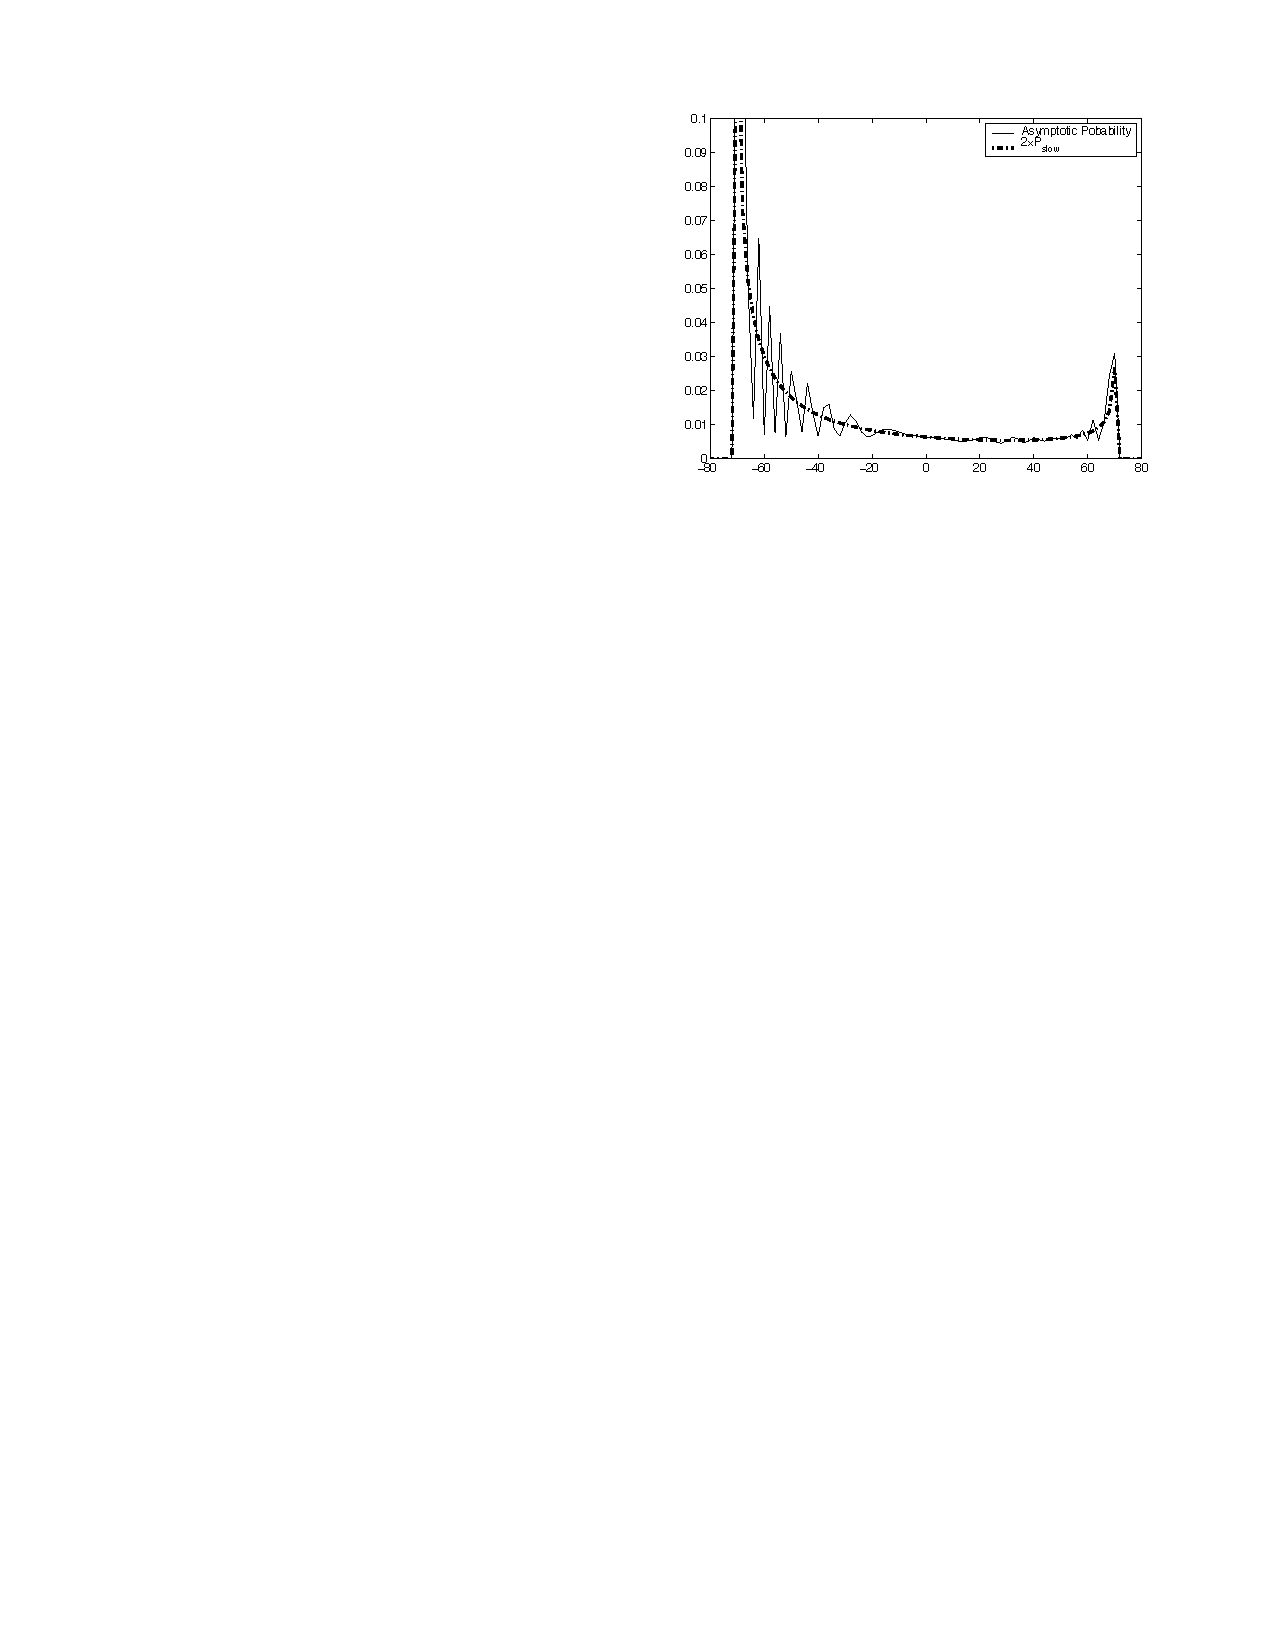
\includegraphics[height=0.6\textheight]{1d_hadamard_quantum_walk.pdf}
    \caption{一維離散Hadamard量子遊走位置狀態概率分布}
  \end{figure}
\end{frame}

\begin{frame}
  \frametitle{測試表格}  
\begin{table}
    \centering
  	\begin{tabular}{|c||c|c|c|c|c|c|c|c|c|c|c|}
    \hline
      \cell{1em}{1em}{$n$} 
    & \cell{1em}{1em}{$-5$} 
    & \cell{1em}{1em}{$-4$} 
    & \cell{1em}{1em}{$-3$} 
    & \cell{1em}{1em}{$-2$}
    & \cell{1em}{1em}{$-1$}
    & \cell{1em}{1em}{$0$}
    & \cell{1em}{1em}{$1$} 
    & \cell{1em}{1em}{$2$} 
    & \cell{1em}{1em}{$3$} 
    & \cell{1em}{1em}{$3$} 
    & \cell{1em}{1em}{$5$} \\ 
    \hline
      $0$ & & & & & & $1$ & & & & & \\ 
    \hline	
      $1$ & & & & & $\frac{1}{2}$ & & $\frac{1}{2}$ & & & & \\ 
    \hline
      $2$ & & & & $\frac{1}{4}$  & & $\frac{2}{4}$ & & $\frac{1}{4}$ & & & \\ 
    \hline
      $3$ & & & $\frac{1}{8}$ & & $\frac{5}{8}$ & & $\frac{1}{8}$ & & $\frac{1}{8}$ & & \\ 
    \hline
      $4$ & & $\frac{1}{16}$ & & $\frac{10}{16}$ & & $\frac{2}{16}$ & & $\frac{2}{16}$ & & $\frac{1}{16}$ & \\ 
    \hline
      $5$ & $\frac{1}{32}$ & & $\frac{17}{32}$ & & $\frac{4}{32}$ & & $\frac{4}{32}$& & $\frac{5}{32}$ & & $\frac{1}{32}$ \\    
    \hline
  	\end{tabular}
    \caption{一維離散Hadamard量子遊走在經過$5$步後的位置概率分布}
	\end{table} 
\end{frame}

%%%%%%%%%%%%%%%%%%%%%%%%%%%%%%%%%%%%%%%%%%%%%%%%%%%%%%%%%%%%%%%%%%%%%%%%%%%%%%%
\end{document}
